%%%%%%%%%%%%%%%%%%%% book.tex %%%%%%%%%%%%%%%%%%%%%%%%%%%%%
%
% sample root file for the chapters of your "monograph"
%
% Use this file as a template for your own input.
%
%%%%%%%%%%%%%%%% Springer-Verlag %%%%%%%%%%%%%%%%%%%%%%%%%%


% RECOMMENDED %%%%%%%%%%%%%%%%%%%%%%%%%%%%%%%%%%%%%%%%%%%%%%%%%%%
\documentclass[envcountsame,envcountchap]{svmono}


% choose options for [] as required from the list
% in the Reference Guide, Sect. 2.2
\usepackage[portuguese]{babel}
\usepackage{makeidx}         % allows index generation
\usepackage{graphicx}        % standard LaTeX graphics tool
                             % when including figure files
\usepackage{multicol}        % used for the two-column index
\usepackage[bottom]{footmisc}% places footnotes at page bottom
\usepackage[utf8]{inputenc}
%\usepackage[T1]{fontenc}
\usepackage{color}
\usepackage{listings}
\usepackage{float}

% etc.
% see the list of further useful packages
% in the Reference Guide, Sects. 2.3, 3.1-3.3

\makeindex             % used for the subject index
                       % please use the style svind.ist with
                       % your makeindex program


\floatstyle{ruled}
\newfloat{f_exemplo}{!ht}{lop}
\floatname{f_exemplo}{Exemplo}

%%%%%%%%%%%%%%%%%%%%%%%%%%%%%%%%%%%%%%%%%%%%%%%%%%%%%%%%%%%%%%%%%%%%%

\begin{document}

\author{João Filipe Meneses Henriques\\João Nuno Santos de Gusmão Guedes}
\title{Turn 12\\
{\small FEUP-PLOG, Turma 3MIEIC05, Grupo 17}}
\subtitle{-- Monograph --}
\maketitle

\frontmatter%%%%%%%%%%%%%%%%%%%%%%%%%%%%%%%%%%%%%%%%%%%%%%%%%%%%%%

%
%%%%%%%%%%%%%%%%%%%%%%% dedic.tex %%%%%%%%%%%%%%%%%%%%%%%%%%%%%%%%%
%
% sample dedication
%
% Use this file as a template for your own input.
%
%%%%%%%%%%%%%%%%%%%%%%%% Springer-Verlag %%%%%%%%%%%%%%%%%%%%%%%%%%

\thispagestyle{empty}
\vspace*{3.5cm}
\begin{flushright}

% write your text here
{\large Your dedication goes here}

\end{flushright}




%%%%%%%%%%%%%%%%%%%%%%% pref.tex %%%%%%%%%%%%%%%%%%%%%%%%%%%%%%%%%%%%%
%
% sample preface
%
% Use this file as a template for your own input.
%
%%%%%%%%%%%%%%%%%%%%%%%% Springer-Verlag %%%%%%%%%%%%%%%%%%%%%%%%%%

\preface

%% Please write your preface here
Here come the golden words


%% Please "sign" your preface
\vspace{1cm}
\begin{flushright}\noindent
place(s),\hfill {\it First name  Surname}\\
month year\hfill {\it First name  Surname}\\
\end{flushright}




\tableofcontents


\mainmatter%%%%%%%%%%%%%%%%%%%%%%%%%%%%%%%%%%%%%%%%%%%%%%%%%%%%%%%

%%%%%%%%%%%%%%%%%%%%% chapter.tex %%%%%%%%%%%%%%%%%%%%%%%%%%%%%%%%%
%
% sample chapter
%
% Use this file as a template for your own input.
%
%%%%%%%%%%%%%%%%%%%%%%%% Springer-Verlag %%%%%%%%%%%%%%%%%%%%%%%%%%

\chapter{Resumo}
\label{abstract} % Always give a unique label
% use \chaptermark{}
% to alter or adjust the chapter heading in the running head

Este artigo foi elaborado no contexto do curso de Programação em Lógica, e incide sobre a programação em lógica com restrições. 
A programação em lógica com restrições permite restringir problemas por domínio de soluções e por condições que devem ser cumpridas. 

Com o objectivo de avaliar a viabilidade da programação com restrições para resolver problemas de lógica de complexidade relevante, foram desenvolvidos algoritmos de resolução e de geração de novas soluções para dimensões variáveis do jogo Turn 12.
Para o efeito fez-se recurso à biblioteca de restrições para o cojunto dos domínios finitos clp(FD) do SICStus Prolog.

O método utilizado compreende a rotação dos dígitos de cada face, sendo o domínio o conjunto de rotações possíveis. A combinação das faces é feita iterativamente e não simultâneamente, por forma a optimizar os recursos.

Obtiveram-se resultados em tempo útil para solucionar o problema original e para um número de digitos não superior a 60, o que permitiu concluir que a metodologia utilizada é adequada para a resolução de problemas do género.

%%%%%%%%%%%%%%%%%%%%% introduction.tex %%%%%%%%%%%%%%%%%%%%%%%%%%%%%%%%%
%
% Introduction chapter
%
%%%%%%%%%%%%%%%%%%%%%%%% Springer-Verlag %%%%%%%%%%%%%%%%%%%%%%%%%%

\chapter{Conteúdo}
\label{cont}

\section{Introducão}
\label{introduction} % Always give a unique label
% use \chaptermark{}
% to alter or adjust the chapter heading in the running head

Programação em lógica com restrições é uma junção de dois paradigmas: solução de restrições e programação em lógica. Esta combinação permite uma concepção mais expressiva e flexível — e em alguns casos mais eficiente - de problemas lógicos.

\subsection{Motivação}
\label{sec:1}
% Always give a unique label
% and use \ref{<label>} for cross-references
% and \cite{<label>} for bibliographic references
% use \sectionmark{}
% to alter or adjust the section heading in the running head
A motivação deste trabalho incidiu na compreensão de um paradigma de programação que já nos é familiar, envolvendo uma nova componente de restrições; resolver problemas lógicos com restrições de uma forma geral, tendo a possibilidade de os refinar e otimizar para uma solução particular.

\subsection{Objectivos}
\label{sec:2}
Resolver a versão original do jogo Turn12 recorrendo a restrições; gerar cubos com um número de dígitos variável, e avaliar se estes têm solução ou não segundo as restrições definidas.


\section{Descrição do problema}
\label{sec:3}
O problema centra-se num cubo em que cada face contém dígitos numerados de 3 a 9, aleatoriamente. Na junção das arestas de cada face, a soma dos dois dígitos que se encontram deverá ser igual a 12.

A solução original (Fig. \ref{fig:1}) com 24 dígitos por face é única.

Na geração de problemas, a resolução que apresentamos contempla dígitos ilimitados, e uma vez que não existe qualquer padrão associado à sequência de dígitos no problema original, estes são gerados aleatoriamente.

No entanto, para garantir a unicidade de solução, em valores demasiado elevados (superiores a 60 por face), as limitações de computação começaram-se a sentir e torna-se improvável gerar uma solução única em tempo útil.

%Figura cubo
\begin{figure}[H]
\begin{center}
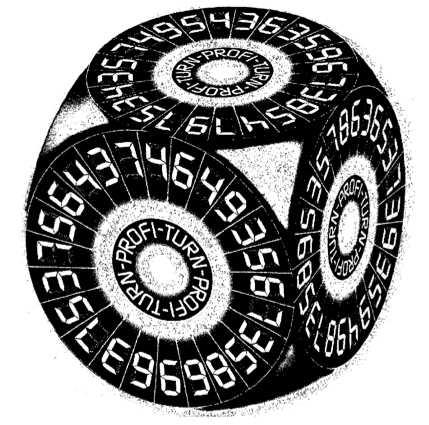
\includegraphics[scale=0.4]{turn12.png}
\caption{Problema original, com os pontos de contacto visíveis assinalados}
\label{fig:1}
\end{center}
\end{figure}



\section{Ficheiros de Dados}
\label{data:1}

Os ficheiros de dados são simples ficheiros de texto (\textit{.txt}), contendo em cada linha os dígitos de cada face.
As faces encontram-se pela seguinte ordem: Topo, Baixo, Frente, Trás, Esquerda e por fim Direita.

De seguida encontra-se um exemplo deste ficheiro com os valores do problema original:

\begin{f_exemplo}[H]
\begin{verbatim}

356735869637537564374649
343574954363596738547975
353748635975458485676439
349576573795398457964379
357863653739359498735895
348765738453874583769785
\end{verbatim}
\caption{Problema original do turn12, com 24 dígitos por face:}
\end{f_exemplo}



\section{Variáveis de Decisão}
\label{restr:1}

As variáveis de decisão usadas na solução foram as rotações que podiam ser feitas em cada face do cubo.\\
Estas rotações têm um domínio compreendido entre 1 e o número de dígitos de cada face.

\section{Restrições}
\label{restr:2}

Independentemente do número de dígitos em cada face, verificou-se que as restrições seriam sempre as mesmas: a soma dos dígitos no ponto de contacto entre duas faces tem de ser 12.\\

Na implementação foi utilizado no \textit{SICStus Prolog} a biblioteca de restrições para o conjunto dos domínios finitos \textit{clp(FD)}, onde foram definidas variáveis que seriam preenchidas com os valores dos pontos de contacto tendo em conta a rotação aplicada sobre cada face, e restringidas de forma a que a soma dos mesmos seja obrigatoriamente 12.

\section{Função de Avaliação}
\label{restr:3}

Os predicados de avaliação chamam-se \textit{turn12}. Foram implementados três com o mesmo nome na solução, mas o principal aceita como parâmetros de entrada as 6 faces do cubo, que deverão ser cada um uma lista numérica de dígitos. Se for encontrada uma solução, são definidos como parâmetros de saída as rotações respectivas de cada face. São também definidos e agrupados 4 a 4 os valores da solução. Este predicado tem como objectivo apenas retornar a primeira solução encontrada.\\
O segundo predicado, com o mesmo nome, tem como parâmetro de entrada a localização do ficheiro com a informação de cada face, e só termina até imprimir todas as soluções do problema.
Por fim, existe ainda um último predicado que não aceita qualquer parâmetro, e que chama o predicado anteriormente descrito, com um ficheiro numa localização predefinida.


\section{Estratégia de Pesquisa}
\label{rest:4}

A estratégia de pesquisa baseia-se na rotação de cada face até encontrar uma solução.
De forma a optimizar a resolução do problema, o algoritmo começa apenas com duas faces, e tenta encontrar através do predicado de etiquetagem \textit{labeling} uma rotação que consiga somar o valor 12 nos seus pontos de contactoo.
Quando encontrada, é passada para outra face do cubo, e com recurso a outro predicado de etiquetagem é tentado encontrar uma rotação para esta última que consiga satisfazer as mesmas restrições para os pontos de contacto em comum com as duas faces anteriores. É seguida sempre a mesma estratégia para as restantes faces, fazendo com que a complexidade algorítmica seja sempre a menor possível.
A razão para a utilização de vários predicados de etiquetagem deve-se ao facto de ser utilizado um predicado auxiliar (\textit{shifted\_face}), que preenche as variáveis utilizadas para testar as restrições com base na rotação correspondente. 
Verificou-se que, quando utilizado um único predicado para o mesmo efeito, o \textit{shifted\_face} era chamado desnecessariamente mesmo para as faces em que a rotação se mantinha igual e que não tinham originado a falha.
Após isolados, o predicado só passou a ser chamado para a face do respectivo labeling, e evitando um varrimento contínuo e dispendioso nas várias listas de dígitos de cada face.

\section{Visualização da Solução}
\label{rest:5}

A visualização da solução é feita através do predicado \textit{project\_cube}.
Este predicado faz uma projecção (Fig. \ref{fig:2}) do cubo de 3 dimensões em 2, e tem como parâmetros de entrada os valores da solução encontrada pelo algorítmo de procura. Estes parâmetros são passados em grupos de 4, representando os pontos de contacto de cada face pela seguinte ordem: ponto superior, direito, inferior e esquerdo. 
A ordem de passagem das faces é : Topo,Traseira, Direita, Esquerda, Dianteira, Inferior.

\begin{figure}[H]
\begin{center}
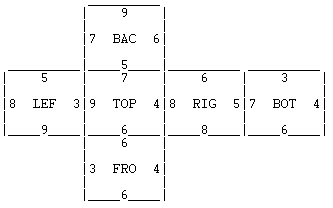
\includegraphics[scale=0.6]{resol.png}
\caption{Impressão da solução do problema original do turn12.}
\label{fig:2}
\end{center}
\end{figure}

Adicionalmente, foi desenvolvido o predicado \textit{print\_rots}, que imprime o número de rotações (Fig. \ref{fig:3})  que devem ser dadas em cada face sobre o problema original para chegar à solução, no sentido contrário ao dos ponteiro do relógio.

\begin{figure}[H]
\begin{center}
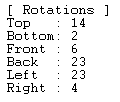
\includegraphics[scale=0.6]{rots.png}
\caption{Impressão das rotações do problema original do turn12.}
\label{fig:3}
\end{center}
\end{figure}


\section{Resultados}
\label{rest:6}

De seguida seguem-se dois exemplos da resolução de dois problemas com complexidades diferentes, gerados com o predicado \textit{turn12gen}

\begin{f_exemplo}[H]
\begin{verbatim}

8987698939348595456596537597964569768569756345737893
6756434375953493785343639458956939579893487543689353
3579793975458794354537534574645348648939348956983756
6789345463497649386734675747959348987858395394783478
4636795348358376783754934938935675854758379538676936
6456984789496935693937974554589635464347893474635735
\end{verbatim}
\caption{Problema com 52 dígitos por face:}
\end{f_exemplo}

\begin{figure}[H]
\begin{center}
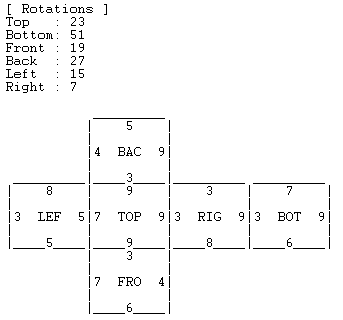
\includegraphics[scale=0.7]{ex1.png}
\caption{Solução do problema com 52 dígitos por face}
\label{fig:4}
\end{center}
\end{figure}

\begin{f_exemplo}[H]
\begin{verbatim}

894896346958797867878397593785997678947876483959373486864543438685698676
739475798946785793456537485839735954538537834873597678963893563438758346
876768685479345693587896839654685468943463769386734938644896978963478579
467998968397969378534737893478583896345647846478475486739653976367948939
469893649494653679565694856947898675395494956976355856784965975784895785
784837634596534396493678394685453865348743489746597473438967439397839853
\end{verbatim}
\caption{Problema com 72 dígitos por face:}
\end{f_exemplo}

\begin{figure}[H]
\begin{center}
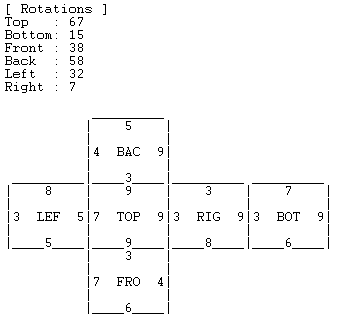
\includegraphics[scale=0.7]{ex2.png}
\caption{Solução do problema com 72 dígitos por face}
\label{fig:4}
\end{center}
\end{figure}



%


%\appendix
%\include{appendix}

\backmatter%%%%%%%%%%%%%%%%%%%%%%%%%%%%%%%%%%%%%%%%%%%%%%%%%%%%%%%
%
\chapter*{Solutions}
\addcontentsline{toc}{chapter}{Solutions}
\markboth{Solutions}{Solutions}

\section*{Problems of Chapter~\ref{intro}}

\begin{sol}{prob1}
The solution is revealed here.
\end{sol}


\begin{sol}{prob2}
\textbf{Problem Heading}\\
(a) The solution of first part is revealed here.\\
(b) The solution of second part is revealed here.
\end{sol}


%%%%%%%%%%%%%%%%%%%%%%%% referenc.tex %%%%%%%%%%%%%%%%%%%%%%%%%%%%%%
% sample references
% "computer science"
%
% Use this file as a template for your own input.
%
%%%%%%%%%%%%%%%%%%%%%%%% Springer-Verlag %%%%%%%%%%%%%%%%%%%%%%%%%%

%
% BibTeX users please use
% \bibliographystyle{}
% \bibliography{}
%
% Non-BibTeX users please use
\begin{thebibliography}{99.}
%
% and use \bibitem to create references.
%
% Use the following syntax and markup for your references
%
% Monographs
\bibitem{monograph} Kajan E (2002)
Information technology encyclopedia and acronyms. Springer, Berlin
Heidelberg New York

% Contributed Works
\bibitem{contribution} Broy M (2002) Software engineering -- From
auxiliary to key technologies. In: Broy M, Denert E (eds)
Software Pioneers. Springer, Berlin Heidelberg New York

% Journal
\bibitem{journal} Che M, Grellmann W, Seidler S (1997)
Appl Polym Sci 64:1079--1090

% Theses
\bibitem{thesis} Ross DW (1977) Lysosomes and storage diseases. MA
Thesis, Columbia University, New York

\end{thebibliography}


\chapter{Anexo}
\label{anex:1}

\lstset{ %
language=Prolog,                % choose the language of the code
basicstyle=\footnotesize,       % the size of the fonts that are used for the code
numbers=left,                   % where to put the line-numbers
numberstyle=\footnotesize,      % the size of the fonts that are used for the line-numbers
stepnumber=1,                   % the step between two line-numbers. If it is 1 each line will be numbered
numbersep=5pt,                  % how far the line-numbers are from the code
backgroundcolor=\color{white},  % choose the background color. You must add \usepackage{color}
commentstyle=\color{blue},
showspaces=false,               % show spaces adding particular underscores
showstringspaces=false,         % underline spaces within strings
showtabs=false,                 % show tabs within strings adding particular underscores
frame=single,   		% adds a frame around the code
tabsize=2,  		% sets default tabsize to 2 spaces
captionpos=b,   		% sets the caption-position to bottom
breaklines=true,    	% sets automatic line breaking
breakatwhitespace=false,    % sets if automatic breaks should only happen at whitespace
escapeinside={\$}{)}         % if you want to add a comment within your code
}


\lstset{literate=%
{á}{{\'a}}1
{Á}{{\'A}}1
{é}{{\'e}}1
{É}{{\'E}}1
{í}{{\'i}}1
{Í}{{\'I}}1
{ó}{{\'o}}1
{Ó}{{\'O}}1
{ú}{{\'u}}1
{Ú}{{\'U}}1
{ç}{{\c{c}}}1
{Ç}{{\c{C}}}1
{ã}{{a}}1
{Ã}{{A}}1
{à}{{\`a}}1
{À}{{\`A}}1
{ê}{{\^e}}1
{Ê}{{\^E}}1
{õ}{{o}}1
{Õ}{{O}}1
}

\section{Turn12}
\label{anex:2}

\lstset{ caption={Código ProLog: turn12.pl}}
\begin{lstlisting}

:- use_module(library(clpfd)).
:- use_module(library(random)).
:- use_module(library(lists)).



not(P) :- call(P), !, fail. 
not(_). 

/**********************************************************
 * Manipulation of file path.
 * defines the main path folder, needed in windows
 * or the installation folder of prolog will be used
 **********************************************************/
 
% uncommet to ignore
%main_path('').
main_path('C:/Users/João Henriques/Desktop/Eng. Informática/FEUP/PLOG/turn12/src/').

construct_full_file_path(File, Path) :-
	main_path(Dir),
	atom_concat(Dir, File, Path).
	
	
/**********************************************************
 * Gets and Sets the elements of the list, in pre marked
 * positions, as the new contact points
 **********************************************************/
 
get_elements_pos( _,  _, -1,-1,-1,-1,   A,B,C,D,   A,B,C,D   ):-!.
get_elements_pos( [X|T],  Pos,  Pos,P2,P3,P4,   _,B,C,D,   E,F,G,H   ) :- !,
	Pos1 is Pos - 1,
	get_elements_pos( T,  Pos1,  -1,P2,P3,P4,   X,B,C,D,   E,F,G,H   ).
get_elements_pos( [X|T],  Pos,  P1,Pos,P3,P4,   A,_,C,D,   E,F,G,H   ) :- !,
	Pos1 is Pos - 1,
	get_elements_pos( T,  Pos1,  P1,-1,P3,P4,   A,X,C,D,   E,F,G,H   ).
get_elements_pos( [X|T],  Pos,  P1,P2,Pos,P4,   A,B,_,D,   E,F,G,H   ) :- !,
	Pos1 is Pos - 1,
	get_elements_pos( T,  Pos1,  P1,P2,-1,P4,   A,B,X,D,   E,F,G,H   ).
get_elements_pos( [X|T],  Pos,  P1,P2,P3,Pos,   A,B,C,_,   E,F,G,H   ) :- !,
	Pos1 is Pos - 1,
	get_elements_pos( T,  Pos1,  P1,P2,P3,-1,   A,B,C,X,   E,F,G,H   ).
get_elements_pos( [_|T],  Pos,  P1,P2,P3,P4,   A,B,C,D,   E,F,G,H   ) :- !,
	Pos1 is Pos - 1,
	get_elements_pos( T,  Pos1,  P1,P2,P3,P4,   A,B,C,D,   E,F,G,H   ).

	
/**********************************************************
 * Calculates the positions of new contact points based in
 * input shift.
 **********************************************************/

shifted_face( Face, Shift, TotalElements, Distance, C1, C2, C3, C4 ) :- !,
	S_F1 is ( Shift mod TotalElements ),
	S_F2 is ( ( Shift + Distance ) mod TotalElements ),
	S_F3 is ( ( Shift + ( 2 * Distance ) ) mod TotalElements ),
	S_F4 is ( ( Shift + ( 3 * Distance ) ) mod TotalElements ),
	TotalElementsIn is TotalElements - 1,
	get_elements_pos( Face,  TotalElementsIn,   S_F1,S_F2,S_F3,S_F4,  0,0,0,0,  C1,C2,C3,C4 ).

	
/**********************************************************
 * Prints rotations
 **********************************************************/
	
print_rots(R1,R2,R3,R4,R5,R6) :-
	write('[ Rotations ]'), nl,
	write('Top   : '), write( R1 ), nl,
	write('Bottom: '), write( R2 ), nl,
	write('Front : '), write( R3 ), nl,
	write('Back  : '), write( R4 ), nl,
	write('Left  : '), write( R5 ), nl,
	write('Right : '), write( R6 ), nl.

	
/**********************************************************
 * Converts a list of numbered characters, defined
 * with "", to its numeric value
 **********************************************************/
 
string_to_list(String,ListOut):-!,
	string_to_list(String,[],ListOut).
string_to_list([H|T],ListIn,ListOut):-!,
	Val is H - 48, % o número zero tem o código ascii 48
	string_to_list(T,[Val|ListIn],ListOut).
string_to_list(_,List,List):-!.


/**********************************************************
 * Prints a 2D projection of the cube
 **********************************************************/

w_top_line:- write(' _________').
w_top_line_f:- write('_________').
w_side_space:- write('          ').
w_top_bot_num(N):-write('|    '),write(N),write('    ').
w_bot_num_line(N):- write('|____'),write(N),write('____').
w_empty_line:- write('|         ').
w_middle_nums(TREE_L_DESC,N1,N2):- write('|'),write(N1),write('  ') , write(TREE_L_DESC), write('  '),write(N2).
w_cube_end:-write('|').

project_cube(  TT_C1,TT_C2,TT_C3,TT_C4,   BA_C1,BA_C2,BA_C3,BA_C4,   RR_C1,RR_C2,RR_C3,RR_C4,
               LL_C1,LL_C2,LL_C3,LL_C4,   FF_C1,FF_C2,FF_C3,FF_C4,   BO_C1,BO_C2,BO_C3,BO_C4 ) :-
	
	%                                   BACK
	w_side_space,                       w_top_line,                         nl,
	w_side_space,                       w_top_bot_num(BA_C1),               w_cube_end, nl,
	w_side_space,                       w_empty_line,                       w_cube_end, nl,
	w_side_space,                       w_middle_nums('BAC', BA_C4, BA_C2), w_cube_end, nl,
	w_side_space,                       w_empty_line,                       w_cube_end, nl,
	w_top_line,                         w_bot_num_line(BA_C3),w_cube_end,   w_top_line_f,                      w_top_line, nl,
	
	% LEFT                              TOP                                 RIGHT                               BOTTOM
	w_top_bot_num(LL_C1),               w_top_bot_num(TT_C1),               w_top_bot_num(RR_C1),               w_top_bot_num(BO_C1),               w_cube_end, nl,
	w_empty_line,                       w_empty_line,                       w_empty_line,                       w_empty_line,                       w_cube_end, nl,
	w_middle_nums('LEF', LL_C4, LL_C2), w_middle_nums('TOP', TT_C4, TT_C2), w_middle_nums('RIG', RR_C4, RR_C2), w_middle_nums('BOT', BO_C4, BO_C2), w_cube_end, nl,
	w_empty_line,                       w_empty_line,                       w_empty_line,                       w_empty_line,                       w_cube_end, nl,
	w_bot_num_line(LL_C3),              w_bot_num_line(TT_C3),              w_bot_num_line(RR_C3),              w_bot_num_line(BO_C3),              w_cube_end, nl,
	
	%                                   FRONT
	w_side_space,                       w_top_bot_num(FF_C1),               w_cube_end, nl,
	w_side_space,                       w_empty_line,                       w_cube_end, nl,
	w_side_space,                       w_middle_nums('FRO', FF_C4, FF_C2), w_cube_end, nl,
	w_side_space,                       w_empty_line,                       w_cube_end, nl,
	w_side_space,                       w_bot_num_line(FF_C3),              w_cube_end, nl.
	

/**********************************************************
 * Processes an input file
 **********************************************************/

 processStreamLine(Stream, ListIn, ListOut) :-
	at_end_of_line(Stream), !,
	skip_line(Stream),
	ListOut = ListIn.
processStreamLine(Stream, ListIn, ListOut) :-
	peek_code(Stream, Code),
	Code = -1, !,
	skip_line(Stream),
	ListOut = ListIn. 
processStreamLine(Stream, ListIn, ListOut) :-
	at_end_of_stream(Stream), !,
	ListOut = ListIn.
processStreamLine(Stream, ListIn, ListOut) :-
	get_code(Stream, Code),
	%write(Code), write(','),
	Number is Code - 48,
	Number >= 3,
	Number =< 9, !,
	processStreamLine(Stream, [Number|ListIn], ListOut).
processStreamLine(Stream,_,_):-!,
	write('Os valores aceites para as faces têm de estar 3 e 9, inclusive.'), nl,
	close(Stream),
	abort.
	
parse_file(Filename, Top, Bottom, Front, Back, Left, Right) :-
	open(Filename, read, Stream),
	processStreamLine(Stream, [], Top),
	processStreamLine(Stream, [], Bottom),
	processStreamLine(Stream, [], Front),
	processStreamLine(Stream, [], Back),
	processStreamLine(Stream, [], Left),
	processStreamLine(Stream, [], Right),
	close(Stream).
	
	
/**********************************************************
 * Verifies if all list faces, have the same length
 **********************************************************/
 
verifyLinesLength(Top, Bottom, Front, Back, Left, Right, ToElements):-
	length(Top   , ToElements),
	length(Bottom, L2),
	length(Front , L3),
	length(Back  , L4),
	length(Left  , L5),
	length(Right , L6),
	ToElements = L2,
	ToElements = L3,
	ToElements = L4,
	ToElements = L5,
	ToElements = L6, !.
verifyLinesLength(_,_,_,_,_,_,_):-!,
	write('Not all lines have the same with. Aborting.'), nl,
	abort.

	
/**********************************************************
 * Verifies if the length is a multiple of 4
 **********************************************************/
 
verifyLineDistance(Size, Distance):-
	Size mod 4 =:= 0, !,
	Distance is floor(Size / 4).
verifyLineDistance(_, _):-!,
	write('The lenght of the lines is not a multiple of 4. Aborting.'), nl,
	abort.

	
/**********************************************************
 * turn12 processing
 **********************************************************/

turn12p:-
	turn12('cubo_a.txt').
	
turn12(Filename):-
	construct_full_file_path( Filename, FilePath ),
	not(turn12_all_poss(FilePath)), write(' no'), nl, nl,
	fd_statistics.
 
/*dump_o_face( Top,Bottom,Front,Back,Left,Right, R1,R2,R3,R4,R5,R6 ) :- !,
	length(Top, Size),
	S1 is Size - R1,
	S2 is Size - R2,
	S3 is Size - R3,
	S4 is Size - R4,
	S5 is Size - R5,
	S6 is Size - R6,
	shuffle_cube_face( Top   , S1, ShuffTop    ),
	shuffle_cube_face( Bottom, S2, ShuffBottom ),
	shuffle_cube_face( Front , S3, ShuffFront  ),
	shuffle_cube_face( Back  , S4, ShuffBack   ),
	shuffle_cube_face( Left  , S5, ShuffLeft   ),
	shuffle_cube_face( Right , S6, ShuffRight  ),
	write_cube_file('C:/Users/João Henriques/Desktop/Eng. Informática/FEUP/PLOG/turn12/src/cubo_a_t.txt',
		ShuffTop, ShuffBottom, ShuffFront, ShuffBack, ShuffLeft, ShuffRight ).*/

turn12( Top, Bottom, Front, Back, Left, Right,    R1, R2, R3, R4, R5, R6,
		TT_C1,TT_C2,TT_C3,TT_C4,   BO_C1,BO_C2,BO_C3,BO_C4,    FF_C1,FF_C2,FF_C3,FF_C4,
		BA_C1,BA_C2,BA_C3,BA_C4,   LL_C1,LL_C2,LL_C3,LL_C4,    RR_C1,RR_C2,RR_C3,RR_C4  ) :-
	
	verifyLinesLength(Top, Bottom, Front, Back, Left, Right, TotElems),
	verifyLineDistance( TotElems, Distance ),

	Rotations = [ R1, R2, R3, R4, R5, R6 ],

	domain(Rotations, 1, TotElems),

	
	% os labelings foram separados de forma a evitar que o predicado shifted_face
	% seja corrido sem ser necessário. Desta forma sempre que um shifted_face falha,
	% volta ao labeling anterior, e gera a rotação da face, só voltando aos labelings
	% anteriores assim que o mesmo esgota todas as possibilidades do domínio.
	
	% Face Topo com a face de Trás
	TT_C1 + BA_C3 #= 12,
	
	labeling([], [R1,R4]),
	shifted_face( Top   , R1, TotElems, Distance, TT_C1, TT_C2, TT_C3, TT_C4 ),
	shifted_face( Back  , R4, TotElems, Distance, BA_C1, BA_C2, BA_C3, BA_C4 ),
	
	
	% Face Topo, com Direira e Trás 
	TT_C2 + RR_C4 #= 12,
	RR_C1 + BA_C2 #= 12,
	
	labeling([], [R6]),
	shifted_face( Right , R6, TotElems, Distance, RR_C1, RR_C2, RR_C3, RR_C4 ),
	

	% Face Topo, com Esquerda e Trás
	TT_C4 + LL_C2 #= 12,
	LL_C1 + BA_C4 #= 12,
	
	labeling([], [R5]),
	shifted_face( Left  , R5, TotElems, Distance, LL_C1, LL_C2, LL_C3, LL_C4 ),

	
	% Face Topo, com Frente, Direita, Esquerda e Trás
	TT_C3 + FF_C1 #= 12,
	RR_C3 + FF_C2 #= 12,
	LL_C3 + FF_C4 #= 12,
	
	labeling([], [R3]),
	shifted_face( Front , R3, TotElems, Distance, FF_C1, FF_C2, FF_C3, FF_C4 ),


	% Face de Baixo com o pontos de contacto das faces adjecentes
	BO_C3 + FF_C3 #= 12,
	BO_C2 + LL_C4 #= 12,
	BO_C4 + RR_C2 #= 12,
	BO_C1 + BA_C1 #= 12,
	
	labeling([], [R2]),
	shifted_face( Bottom, R2, TotElems, Distance, BO_C1, BO_C2, BO_C3, BO_C4 ).

turn12_all_poss(Filename) :-
	write('Reading cube file...'),nl,
	parse_file(Filename, Top, Bottom, Front, Back, Left, Right), !,
	
	write('Attempting to solve cube...'),nl,
	turn12( Top,Bottom,Front,Back,Left,Right,    R1, R2, R3, R4, R5, R6,
			TT_C1,TT_C2,TT_C3,TT_C4,   BO_C1,BO_C2,BO_C3,BO_C4,    FF_C1,FF_C2,FF_C3,FF_C4,
			BA_C1,BA_C2,BA_C3,BA_C4,   LL_C1,LL_C2,LL_C3,LL_C4,    RR_C1,RR_C2,RR_C3,RR_C4   ),

	nl,	print_rots( R1,R2,R3,R4,R5,R6 ), nl,
	
	project_cube( TT_C1,TT_C2,TT_C3,TT_C4,   BA_C1,BA_C2,BA_C3,BA_C4,   RR_C1,RR_C2,RR_C3,RR_C4,
                  LL_C1,LL_C2,LL_C3,LL_C4,   FF_C1,FF_C2,FF_C3,FF_C4,   BO_C1,BO_C2,BO_C3,BO_C4 ),
				  
	%dump_o_face( Top,Bottom,Front,Back,Left,Right,    R1, R2, R3, R4, R5, R6 ),!,
	
	nl,nl,

	write('More possibilities ?'),
	fail. % falha para verificar se existem mais possibilidades	
	
	
	
	
/**********************************************************
 **********************************************************
 * Generating problems
 **********************************************************
 **********************************************************/
 
 
 %
/**********************************************************
 * Generate random number in the domain of the problem
 * [3, 10-1]
 **********************************************************/
 
random_turn12_n(Number):-
	random(3, 10, Number).
	
	
/**********************************************************
 * Guarantees there is no adjecent repeated
 * numbers in each face
 **********************************************************/
 
no_equal_number(N,N, Out) :-!,
	Out is 3 + ( ( ( N + 1 ) - 3 ) mod 7 ).
no_equal_number(_,N,N):-!.	


/**********************************************************
 * Guarantees there is not another not another pattern
 * equal to the original
 **********************************************************/
 
no_equal_pattern( C1,C2,C3,C4, C1,C2,C3,C4, O4 ) :-!,
	no_equal_number(C4, C4, O4).
no_equal_pattern( _,_,_,_,  _,_,_,T4,  T4 ).


/**********************************************************
 * Fills the cube with random numbers in the domain
 * of the problem
 **********************************************************/

fill_cube_face_int(  _,_,_,_,  DistBetweenElems,DistBetweenElems,   A,B,C,D,   FaceOut ) :- !,
	append([], D, L1),
	append(L1, C, L2),
	append(L2, B, L3),
	append(L3, A, FaceOut).
fill_cube_face_int( C1,C2,C3,C4,  Pos,DistBetweenElems,   [HA|A],[HB|B],[HC|C],[HD|D],   FaceOut ) :-
	random_turn12_n( V1_temp ),
	no_equal_number( HA, V1_temp, V1 ),
		
	random_turn12_n( V2_temp ),
	no_equal_number( HB, V2_temp, V2 ),
	
	random_turn12_n( V3_temp ),
	no_equal_number( HC, V3_temp, V3 ),
	
	random_turn12_n( V4_temp ),
	no_equal_number( HD, V4_temp, V4_tt2 ),

	no_equal_pattern( C1,C2,C3,C4,  V1,V2,V3,V4_tt2, V4 ),
	
	NextPos is Pos + 1,
	fill_cube_face_int(  C1,C2,C3,C4,  NextPos,DistBetweenElems,   [V1|[HA|A]],[V2|[HB|B]],[V3|[HC|C]],[V4|[HD|D]],   FaceOut ).
	
fill_cube_face( C1,C2,C3,C4,  DistBetweenElems,  FaceOut ) :-
	fill_cube_face_int( C1,C2,C3,C4,  1,   DistBetweenElems,   [C1],[C2],[C3],[C4],   FaceOut ).	


/**********************************************************
 * Writes the cube face to the file Stream
 **********************************************************/
 
write_cube_line([], _):-!.
write_cube_line([H|T], Stream) :-
	Char is H + 48, % ascii character 0 is 48
	put_code(Stream, Char), !,
	write_cube_line(T, Stream).
write_cube_line(_, Stream) :- !,
	write('Error writing in file. Aborting.'), nl,
	close(Stream),
	abort.
	
	
/**********************************************************
 * Writes the cube faces to file (one per line) in this
 * order: Top, Bottom, Front, Back, Left, Right, 
 **********************************************************/
 
write_cube_file(Filename, Top, Bottom, Front, Back, Left, Right) :-
	open(Filename, write, Stream), !,
	reverse(Top   ,Top_r   ),
	reverse(Bottom,Bottom_r),
	reverse(Front ,Front_r ),
	reverse(Back  ,Back_r  ),
	reverse(Left  ,Left_r  ),
	reverse(Right ,Right_r ),
	write_cube_line(Top_r   , Stream), nl(Stream),
	write_cube_line(Bottom_r, Stream), nl(Stream),
	write_cube_line(Front_r , Stream), nl(Stream),
	write_cube_line(Back_r  , Stream), nl(Stream),
	write_cube_line(Left_r  , Stream), nl(Stream),
	write_cube_line(Right_r , Stream),
	close(Stream).
	
	
/**********************************************************
 * Predicate that only accepts a cube with a unique
 * solution. This is possible because the algorithm that
 * solves the cube starts with a shift of one, if no other
 * solution is found, the solution will have all six
 * rotations with the length of the face.
 **********************************************************/
 
turn12_unique_gen( Top, Bottom, Front, Back, Left, Right ) :- !,
	turn12( Top, Bottom, Front, Back, Left, Right,    R1, R2, R3, R4, R5, R6,
		_,_,_,_,  _,_,_,_,  _,_,_,_,  _,_,_,_,  _,_,_,_,  _,_,_,_  ),
	!,	
	%print_rots(R1,R2,R3,R4,R5,R6),
	length( Top, TotalElem ),	
	R1 = TotalElem,
	R2 = TotalElem,
	R3 = TotalElem,
	R4 = TotalElem,
	R5 = TotalElem,
	R6 = TotalElem.


/**********************************************************
 * Rotates the face list, many times specified.
 **********************************************************/
 
shuffle_cube_face( Face, ShufflePos, FaceOut ) :-
	shuffle_cube_face( Face, 0, ShufflePos, [], FaceOut ).
shuffle_cube_face( [H|T], Pos, ShufflePos, ListIn, FaceOut ) :-
	Pos < ShufflePos,
	append( ListIn, [H], NewList ),
	NewPos is Pos + 1,
	shuffle_cube_face( T, NewPos, ShufflePos, NewList, FaceOut ).
shuffle_cube_face( Tail, _, _, ListIn, FaceOut ) :-
	append( Tail, ListIn, FaceOut ).
	
	
/**********************************************************
 * Rotates the face with a random number
 **********************************************************/
 
randomly_suffle_face( Face, FaceSize, FaceOut ) :-
	random(0, FaceSize, Rotation),
	shuffle_cube_face( Face, Rotation, FaceOut ).
	
	
/**********************************************************
 * Analytics predicates. Just check the sum of each line.
 * Not needed to solve the problem
 **********************************************************/
 
sum_face([], Sum, Sum).
sum_face([H|T], SumIn, SumOut) :-
	NewSum is SumIn + H,
	sum_face(T, NewSum, SumOut).
	
print_face_stats(F,Sum,FSize):-
	Div is Sum / FSize,
	write('    '), write(F), write(' sum is: '), write( Sum ), write(' ('), write(Div), write(')'), nl.
	
print_cube_stats( Top, Bottom, Front, Back, Left, Right, FaceSize ) :-
	sum_face(Top, 0, SumTop),
	sum_face(Back, 0, SumBack),
	sum_face(Right, 0, SumRight),
	sum_face(Left, 0, SumLeft),
	sum_face(Front, 0, SumFront),
	sum_face(Bottom, 0, SumBottom),
	print_face_stats('Top', SumTop, FaceSize),
	print_face_stats('Back', SumBack, FaceSize),
	print_face_stats('Right', SumRight, FaceSize),
	print_face_stats('Left', SumLeft, FaceSize),
	print_face_stats('Front', SumFront, FaceSize),
	print_face_stats('Bottom', SumBottom, FaceSize),
	TotalSum is SumTop + SumBack + SumRight + SumLeft + SumFront + SumBottom,
	print_face_stats('Total', TotalSum, FaceSize).
	
	
/**********************************************************
 * Generates a new problem base on the arguments
 **********************************************************/

turn12gen(Dist):-
	turn12gen( 'cubo_a.txt', Dist ).

turn12gen(Filename, Distance):-
	Distance > 0,
	
	construct_full_file_path( Filename, FilePath ),
	
	repeat,
	write('Making an attempt to find if current generated random numbers can make a solution...'), nl,
	
	random_turn12_n( TT_C1 ),
	random_turn12_n( TT_C2 ),

	random_turn12_n( BO_C1 ),
	random_turn12_n( BO_C3 ),

	random_turn12_n( BA_C2 ),
	random_turn12_n( BA_C4 ),
	
	random_turn12_n( FF_C2 ),
	random_turn12_n( FF_C4 ),
	
	random_turn12_n( LL_C2 ),
	random_turn12_n( LL_C4 ),
	
	random_turn12_n( RR_C2 ),
	random_turn12_n( RR_C4 ),

	ContactPoints = [  TT_C2,TT_C4,    FF_C1,FF_C3,    LL_C2,LL_C4,
                       BO_C2,BO_C4,    BA_C1,BA_C3,    RR_C2,RR_C4   ],

	domain(ContactPoints, 3, 9),
	
	% têm de ser diferentes, se não, ao girar a face 180 graus,
	% e se os cantos opostos forem os mesmos, originaria uma nova solução
	% se os quatro forem iguais, originariam 4 novas soluções.
	TT_C1 #\= TT_C3   #\/   TT_C2 #\= TT_C4,
	BO_C1 #\= BO_C3   #\/   BO_C2 #\= BO_C4,
	
	FF_C1 #\= FF_C3   #\/   FF_C2 #\= FF_C4,
	BA_C1 #\= BA_C3   #\/   BA_C2 #\= BA_C4,
	RR_C1 #\= RR_C3   #\/   RR_C2 #\= RR_C4,
	LL_C1 #\= LL_C3   #\/   LL_C2 #\= LL_C4,

	TT_C1 + BA_C3 #= 12,
		
	TT_C2 + RR_C4 #= 12,
	RR_C1 + BA_C2 #= 12,
	
	TT_C4 + LL_C2 #= 12,
	LL_C1 + BA_C4 #= 12,

	TT_C3 + FF_C1 #= 12,
	RR_C3 + FF_C2 #= 12,
	LL_C3 + FF_C4 #= 12,

	BO_C3 + FF_C3 #= 12,
	BO_C2 + LL_C4 #= 12,
	BO_C4 + RR_C2 #= 12,
	BO_C1 + BA_C1 #= 12,
	
	labeling([], ContactPoints),
	
	repeat,
	
	write('Attempting to fill cube with a unique solution...'), nl,
	fill_cube_face( TT_C1,TT_C2,TT_C3,TT_C4, Distance, Top    ),
	fill_cube_face( BA_C1,BA_C2,BA_C3,BA_C4, Distance, Back   ),
	fill_cube_face( RR_C1,RR_C2,RR_C3,RR_C4, Distance, Right  ),
	fill_cube_face( LL_C1,LL_C2,LL_C3,LL_C4, Distance, Left   ),
	fill_cube_face( FF_C1,FF_C2,FF_C3,FF_C4, Distance, Front  ),
	fill_cube_face( BO_C1,BO_C2,BO_C3,BO_C4, Distance, Bottom ),
	
	FaceSize is Distance * 4,
	
	turn12_unique_gen( Top, Bottom, Front, Back, Left, Right ), !,
	write('Cube has a unique solution.'),nl,
	

	randomly_suffle_face( Top   , FaceSize, ShuffTop    ),
	randomly_suffle_face( Back  , FaceSize, ShuffBack   ),
	randomly_suffle_face( Right , FaceSize, ShuffRight  ),
	randomly_suffle_face( Left  , FaceSize, ShuffLeft   ),
	randomly_suffle_face( Front , FaceSize, ShuffFront  ),
	randomly_suffle_face( Bottom, FaceSize, ShuffBottom ),
	
	project_cube( TT_C1,TT_C2,TT_C3,TT_C4,   BA_C1,BA_C2,BA_C3,BA_C4,   RR_C1,RR_C2,RR_C3,RR_C4,
                  LL_C1,LL_C2,LL_C3,LL_C4,   FF_C1,FF_C2,FF_C3,FF_C4,   BO_C1,BO_C2,BO_C3,BO_C4 ),
				  
	nl, write('Writing cube to file.'), nl,
	write_cube_file(FilePath, ShuffTop, ShuffBottom, ShuffFront, ShuffBack, ShuffLeft, ShuffRight ),
	nl,nl,
	fd_statistics.

turn12gen(_,_):-
	write('Distance between elements must be grater than 0. Aborting.').
	
\end{lstlisting}
%\printindex

%%%%%%%%%%%%%%%%%%%%%%%%%%%%%%%%%%%%%%%%%%%%%%%%%%%%%%%%%%%%%%%%%%%%%%

\end{document}





